\documentclass[11pt,aspectratio=169]{beamer}
\usepackage{amsmath,amssymb,bm,graphicx,booktabs,tikz,pgfplots}
\pgfplotsset{compat=1.17}
\usetikzlibrary{arrows.meta,positioning}

\usetheme{default}
\setbeamertemplate{navigation symbols}{}
\setbeamertemplate{headline}{}
\setbeamertemplate{footline}{}
\setbeamertemplate{frametitle}{\vspace{0.25cm}\insertframetitle\par\vspace{0.08cm}\hrule}
\setbeamercolor{normal text}{fg=black,bg=white}
\setbeamercolor{frametitle}{fg=black,bg=white}
\setbeamercolor{structure}{fg=black}
\setbeamersize{text margin left=0.7cm,text margin right=0.7cm}

\newcommand{\dd}{\,\mathrm{d}}
\newcommand{\Om}{\Omega}
\newcommand{\Gam}{\Gamma}
\newcommand{\R}{\mathbb R}
\newcommand{\Th}{\mathcal T_h}
\newcommand{\Vzero}{\mathcal V_0}
\newcommand{\Vhzero}{\mathcal V_{h,0}}
\newcommand{\Ih}{\mathcal I_h}
\newcommand{\Ie}{\mathcal I_e}
\newcommand{\norm}[2][]{\left\lVert#2\right\rVert_{#1}}
\newcommand{\seminorm}[2][]{\left\lvert#2\right\rvert_{#1}}
\newcommand{\bx}{\bm x}
\newcommand{\bu}{\bm u}
\newcommand{\bv}{\bm v}
\newcommand{\beps}{\bm\varepsilon}

% Frozen output of Chapter 7, Example 7.5, copied here for reproducibility.
\graphicspath{{figures/}}

\begin{document}

\begin{frame}[plain]
  \centering\vfill
  {\LARGE\bfseries A Priori Error Analysis\par}
  \vspace{0.45cm}
  {\large Convergence rates, duality, and numerical verification\par}
  \vfill
\end{frame}

\section{From interpolation to convergence}

\begin{frame}{Starting point from the previous lecture}
For $u\in H^s(\Om)$ with $2\leq s\leq p+1$, the previous lecture established
\[
  \norm[a]{u-u_h}=O(h^{s-1}),
  \qquad
  \norm[H^1(\Om)]{u-u_h}=O(h^{s-1}).
\]
The immediate consequence
\[
  \norm[L^2(\Om)]{u-u_h}
  \leq\norm[H^1(\Om)]{u-u_h}
\]
also gives an $L^2$ bound of order $h^{s-1}$.

The interpolation error is one order smaller in $L^2$:
\[
  \norm[L^2(\Om)]{u-\Ih u}=O(h^s).
\]
The first goal of this lecture is to determine when the finite element
solution has this higher $L^2$ rate.
\end{frame}

\begin{frame}{Lecture outline}
\begin{enumerate}
  \item Identify how polynomial degree and solution regularity limit the
  predicted convergence rates.
  \item Derive the optimal $L^2$ estimate using a dual problem.
  \item Compare predicted rates with errors computed on a mesh sequence.
  \item State the corresponding conclusions for linear elasticity.
\end{enumerate}
\end{frame}

\section{Energy and \texorpdfstring{$H^1$}{H1} convergence}

\begin{frame}{Predicted rates for smooth solutions}
Assume $u\in H^{p+1}(\Om)$. The $L^2$ rates shown in the last column also
require the dual-regularity assumption introduced later.
\par
\vspace{0.2cm}
\centering
\renewcommand{\arraystretch}{1.45}
\begin{tabular}{c|cc}
  \toprule
  degree $p$ & energy and $H^1$ error & $L^2$ error\\
  \midrule
  $1$ & $O(h)$ & $O(h^2)$\\
  $2$ & $O(h^2)$ & $O(h^3)$\\
  $3$ & $O(h^3)$ & $O(h^4)$\\
  \bottomrule
\end{tabular}
\par
\vspace{0.4cm}
$E(h)=O(h^r)$ means $E(h)\leq Ch^r$ with a constant $C$ independent of $h$.
The exponent $r$ is the convergence rate in the selected norm.
\end{frame}

\begin{frame}{Regularity of the exact solution also matters}
\begin{columns}[T,onlytextwidth]
  \begin{column}{0.34\textwidth}
    \centering
    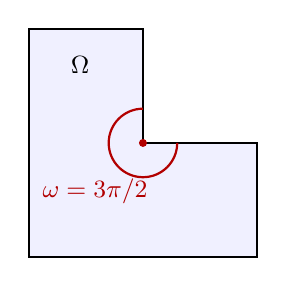
\begin{tikzpicture}[scale=1.45]
      \draw[thick,fill=blue!6]
        (0,0)--(2,0)--(2,1)--(1,1)--(1,2)--(0,2)--cycle;
      \draw[red!70!black,thick]
        (1,1) ++(90:0.3) arc[start angle=90,end angle=360,radius=0.3];
      \fill[red!70!black] (1,1) circle[radius=0.035];
      \node[font=\small,red!70!black] at (0.58,0.58) {$\omega=3\pi/2$};
      \node[font=\small] at (0.45,1.68) {$\Om$};
    \end{tikzpicture}
  \end{column}
  \begin{column}{0.62\textwidth}
    On a polygon with a reentrant corner, the solution of a smooth-data
    Laplace problem may fail to belong to $H^2(\Om)$.
    \vspace{0.25cm}

    The linear-element estimate requires $u\in H^2(\Om)$. If this regularity
    is unavailable, the theorem does not guarantee the usual first-order
    energy convergence.
    \vspace{0.25cm}

    Raising the polynomial degree does not repair missing solution
    regularity. Local refinement near the corner is often more useful;
    Chapter 8 develops a way to decide where refinement is needed.
  \end{column}
\end{columns}
\end{frame}

\begin{frame}{In-class calculation: predict the energy rate}
Assume the hypotheses of the energy-error theorem. Complete the table using
$r=\min(p,s_u-1)$.
\par
\vspace{0.25cm}
\centering
\renewcommand{\arraystretch}{1.55}
\begin{tabular}{c|ccc}
  \toprule
  & $s_u=2$ & $s_u=3$ & $s_u=4$\\
  \midrule
  $p=1$ & & & \\
  $p=2$ & & & \\
  $p=3$ & & & \\
  \bottomrule
\end{tabular}
\par
\vspace{0.4cm}

Why does changing from $p=1$ to $p=3$ not improve the guaranteed rate when
$u\in H^2(\Om)$ but no additional regularity is known?
\end{frame}

\section{\texorpdfstring{$L^2$}{L2} convergence by duality}

\begin{frame}[plain]
  \centering
  \vfill
  {\LARGE\bfseries The optimal $L^2$ estimate\par}
  \vspace{0.45cm}
  {\large A dual problem supplies the additional power of $h$.\par}
  \vfill
\end{frame}

\begin{frame}{Why C\'ea's lemma does not give the optimal $L^2$ rate}
The $H^1$ estimate gives the valid bound
\[
  \norm[L^2(\Om)]{u-u_h}
  \leq\norm[H^1(\Om)]{u-u_h}=O(h^{s-1}).
\]
But one-dimensional examples and the interpolation estimate suggest one
additional power of $h$ in $L^2$.
\vspace{0.25cm}

C\'ea's lemma controls the error in a norm in which the bilinear form is
coercive. For diffusion, that is the energy norm, not the $L^2$ norm.
\vspace{0.25cm}

We therefore introduce an auxiliary problem that converts the squared
$L^2$ error into a bilinear form involving the finite element error.
\end{frame}

\begin{frame}{Step 1: choose the dual problem from the error}
Let $e=u-u_h$. Define the dual solution $z\in\Vzero$ by
\[
  \boxed{a(v,z)=(e,v)_{L^2(\Om)}
  \qquad\forall v\in\Vzero.}
\]
For symmetric diffusion, this is the weak form of
\[
  -\nabla\cdot(k\nabla z)=e\quad\text{in }\Om,
\]
with homogeneous Dirichlet data on $\Gam_D$ and homogeneous flux on
$\Gam_N$.
\vspace{0.2cm}

Taking $v=e$ gives
\[
  \boxed{\norm[L^2(\Om)]{e}^2=a(e,z).}
\]
This identity is the reason for introducing the dual problem.
\end{frame}

\begin{frame}{The extra assumption: dual regularity}
Lax--Milgram gives $z\in\Vzero$, but the interpolation estimate used next
requires $z\in H^2(\Om)$.
\vspace{0.2cm}

We assume
\[
  \boxed{z\in H^2(\Om),
  \qquad
  \seminorm[H^2(\Om)]{z}
  \leq C_{\mathrm{reg}}\norm[L^2(\Om)]{e}.}
\]
This is a property of the domain, coefficient, and boundary partition, not of
the mesh. It holds for many smooth or convex problems, but it can fail at
reentrant corners, across coefficient jumps, or where the boundary-condition
type changes.
\end{frame}

\begin{frame}{Step 2: use Galerkin orthogonality}
Since $z\in H^2(\Om)$, $\Ih z$ is defined and belongs to $\Vhzero$.
Galerkin orthogonality gives
\[
  a(e,\Ih z)=0.
\]
Therefore
\[
  \norm[L^2(\Om)]{e}^2
  =a(e,z)=a(e,z-\Ih z).
\]
\vspace{0.25cm}

The dual solution itself is not small, but its interpolation error is:
\[
  \seminorm[H^1(\Om)]{z-\Ih z}
  \leq C_Ih\seminorm[H^2(\Om)]{z}.
\]
This factor $h$ produces the additional order in the $L^2$ error.
\end{frame}

\begin{frame}{Step 3: bound the two factors}
\begin{align*}
  \norm[L^2(\Om)]{e}^2
  &=a(e,z-\Ih z)\\
  &\leq k_1\seminorm[H^1(\Om)]{e}
    \seminorm[H^1(\Om)]{z-\Ih z}\\
  &\leq k_1C_Ih\seminorm[H^1(\Om)]{e}
    \seminorm[H^2(\Om)]{z}\\
  &\leq k_1C_IC_{\mathrm{reg}}h
    \seminorm[H^1(\Om)]{e}\norm[L^2(\Om)]{e}.
\end{align*}
Dividing by $\norm[L^2(\Om)]{e}$ gives
\[
  \norm[L^2(\Om)]{e}
  \leq k_1C_IC_{\mathrm{reg}}h\seminorm[H^1(\Om)]{e}.
\]
Combining this with the $H^1$ estimate gives
\[
  \boxed{\norm[L^2(\Om)]{u-u_h}=O(h^s).}
\]
For a smooth degree-$p$ approximation, this is $O(h^{p+1})$.
\end{frame}

\begin{frame}{What the duality argument used}
\begin{enumerate}
  \item Choose the dual right-hand side to be $e=u-u_h$.
  \item Use the dual equation to write $\norm[L^2]{e}^2=a(e,z)$.
  \item Use Galerkin orthogonality to replace $z$ by $z-\Ih z$.
  \item Use $H^2$ regularity to bound the dual interpolation error by
  $O(h)\norm[L^2]{e}$.
\end{enumerate}
\vspace{0.35cm}

Without the additional regularity of $z$, Step 4 does not give a full factor
of $h$. The improved $L^2$ rate is conditional, not automatic.
\end{frame}

\section{Numerical verification}

\begin{frame}[plain]
  \centering
  \vfill
  {\LARGE\bfseries Numerical verification\par}
  \vspace{0.45cm}
  {\large Compare predicted rates with errors computed during mesh refinement.\par}
  \vfill
\end{frame}

\begin{frame}{Observed convergence rate}
Suppose $E(h)\approx Ch^r$. For two mesh sizes $h_1>h_2$,
\[
  \frac{E(h_1)}{E(h_2)}\approx\left(\frac{h_1}{h_2}\right)^r.
\]
Solving for $r$ gives
\[
  \boxed{r_{\mathrm{obs}}
  =\frac{\log(E(h_1)/E(h_2))}{\log(h_1/h_2)}.}
\]
For uniform refinement with $h_2=h_1/2$,
\[
  r_{\mathrm{obs}}=\log_2\!\left(\frac{E(h)}{E(h/2)}\right).
\]
An error reduction by factors $2$, $4$, and $8$ corresponds to observed
rates $1$, $2$, and $3$, respectively.
\end{frame}

\begin{frame}{A convergence study tests a specific prediction}
A meaningful verification study requires:
\begin{enumerate}
  \item a known smooth solution, often obtained by the method of manufactured
  solutions;
  \item a mesh sequence satisfying the assumptions of the estimate;
  \item the error measured in the norm for which a rate is predicted;
  \item sufficiently accurate quadrature for the error integrals; and
  \item several refinements in the asymptotic range.
\end{enumerate}
\vspace{0.3cm}

Errors sampled only at the nodes are not sufficient. In some one-dimensional
problems, the finite element nodal values are exact even though the error
between nodes is nonzero.
\end{frame}

\begin{frame}{Uniformly loaded bar: exact error rates}
\begin{columns}[T,onlytextwidth]
  \begin{column}{0.53\textwidth}
    \centering
    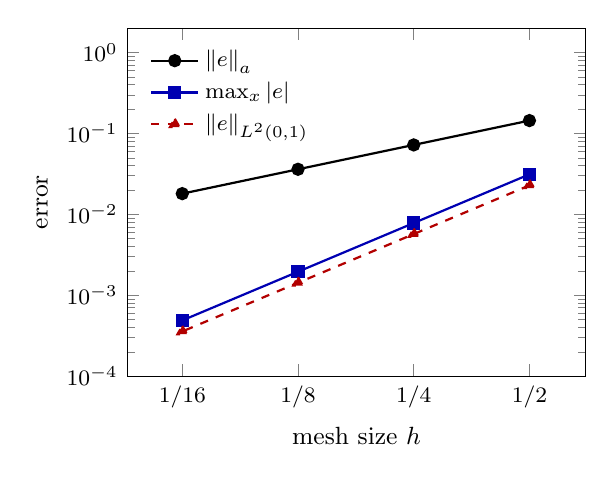
\begin{tikzpicture}
      \begin{axis}[width=7.4cm,height=6.0cm,xmode=log,ymode=log,
        log basis x={2},xmin=0.045,xmax=0.7,ymin=1e-4,ymax=2,
        xtick={0.0625,0.125,0.25,0.5},
        xticklabels={$1/16$,$1/8$,$1/4$,$1/2$},
        xlabel={mesh size $h$},ylabel={error},
        tick label style={font=\footnotesize},label style={font=\small},
        legend pos=north west,
        legend style={font=\footnotesize,draw=none,fill=none},
        legend cell align=left]
        \addplot[thick,mark=*,color=black] coordinates {
          (0.5,1.443e-1)(0.25,7.217e-2)(0.125,3.608e-2)(0.0625,1.804e-2)};
        \addlegendentry{$\norm[a]{e}$}
        \addplot[thick,mark=square*,color=blue!70!black] coordinates {
          (0.5,3.125e-2)(0.25,7.813e-3)(0.125,1.953e-3)(0.0625,4.883e-4)};
        \addlegendentry{$\max_x|e|$}
        \addplot[thick,dashed,mark=triangle*,color=red!70!black] coordinates {
          (0.5,2.282e-2)(0.25,5.705e-3)(0.125,1.426e-3)(0.0625,3.566e-4)};
        \addlegendentry{$\norm[L^2(0,1)]{e}$}
      \end{axis}
    \end{tikzpicture}
  \end{column}
  \begin{column}{0.44\textwidth}
    For $L=AE=f_0=1$,
    \[
      u(x)=x-\frac{x^2}{2},\qquad u_h=\Ih u.
    \]
    The errors are
    \[
      \max_x|e|=\frac{h^2}{8},\qquad
      \norm[L^2(0,1)]{e}=\frac{h^2}{\sqrt{120}},
    \]
    \[
      \norm[a]{e}=\frac{h}{\sqrt{12}}.
    \]
    Halving $h$ divides the energy error by $2$ and the other errors by $4$.
    The observed rates are $1$, $2$, and $2$.
  \end{column}
\end{columns}
\end{frame}

\begin{frame}{Manufactured solution: linear and quadratic elements}
\begin{columns}[T,onlytextwidth]
  \begin{column}{0.60\textwidth}
    \centering
    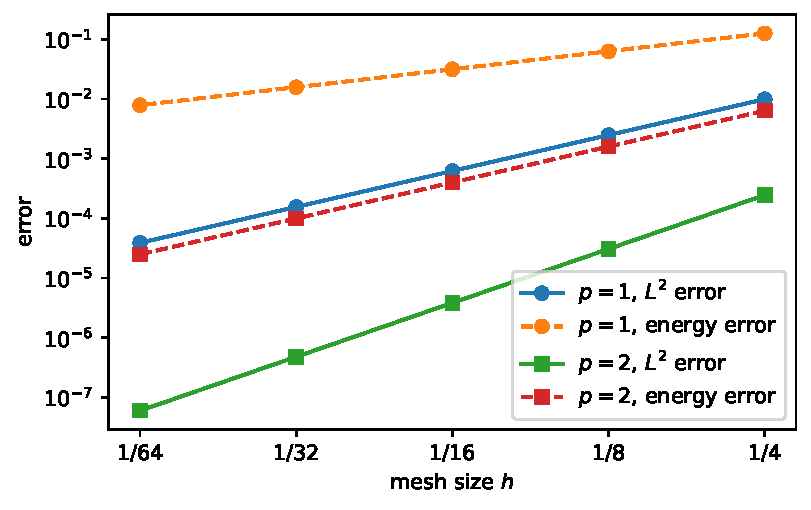
\includegraphics[width=\textwidth]{fig-c7-convergence-rates-output-2.pdf}
  \end{column}
  \begin{column}{0.37\textwidth}
    \small
    The manufactured solution is
    \[
      u(x)=\sin\frac{\pi x}{2}\quad\text{on }(0,1).
    \]
    It is smooth and is not reproduced exactly by either approximation.
    \vspace{0.2cm}

    \centering
    \renewcommand{\arraystretch}{1.3}
    \begin{tabular}{c|cc}
      \toprule
      & $L^2$ & energy\\
      \midrule
      $p=1$ & $2.00$ & $1.00$\\
      $p=2$ & $3.00$ & $2.00$\\
      \bottomrule
    \end{tabular}
    \vspace{0.25cm}

    \raggedright These are the predicted rates $p+1$ and $p$.
  \end{column}
\end{columns}
\end{frame}

\begin{frame}{In-class calculation: read a two-dimensional study}
The Chapter 6 diffusion example used $P_1$ triangles and produced the
following integrated $L^2$ errors:
\vspace{0.15cm}

\begin{columns}[T,onlytextwidth]
  \begin{column}{0.42\textwidth}
    \centering
    \renewcommand{\arraystretch}{1.3}
    \begin{tabular}{rcc}
      \toprule
      triangles & $h$ & $L^2$ error\\
      \midrule
      $4$  & $1.118$ & $1.291\times10^{-1}$\\
      $16$ & $0.559$ & $3.870\times10^{-2}$\\
      $64$ & $0.280$ & $1.079\times10^{-2}$\\
      \bottomrule
    \end{tabular}
  \end{column}
  \begin{column}{0.55\textwidth}
    \begin{enumerate}
      \item Compute $r_{\mathrm{obs}}$ for each refinement.
      \item What rate is predicted for a smooth solution with linear
      elements?
      \item Do two observed rates provide convincing verification? What
      additional information or computations would you request?
    \end{enumerate}
  \end{column}
\end{columns}
\end{frame}

\section{Linear elasticity}

\begin{frame}{The same argument applies to linear elasticity}
For homogeneous prescribed displacement data,
\[
  a_{\mathrm{el}}(\bu-\bu_h,\bv_h)=0
  \qquad\forall\bv_h\in\mathcal V_{h,0}.
\]
Continuity, Korn's inequality, and C\'ea's lemma give
\[
  \norm[H^1(\Om;\R^d)]{\bu-\bu_h}
  \leq\frac{C_{\mathbb C}C_K^2}{c_{\mathbb C}}
  \inf_{\bv_h\in\mathcal V_{h,0}}
  \norm[H^1(\Om;\R^d)]{\bu-\bv_h}.
\]
Applying the interpolation estimate componentwise gives
\[
  \norm[H^1(\Om;\R^d)]{\bu-\bu_h}=O(h^{s-1}),
  \qquad 2\leq s\leq p+1.
\]
The strain and stress errors have the same order because they depend on the
first derivatives of displacement.
\end{frame}

\begin{frame}{Energy best approximation and compliance}
When the elasticity tensor has the major symmetry,
\[
  \norm[a_{\mathrm{el}}]{\bv}^2
  =\int_\Om\beps(\bv):\mathbb C:\beps(\bv)\dd\bx
\]
defines the elastic energy norm. The finite element solution is the best
approximation in this norm.

For the continuous and discrete solutions,
\[
  \ell_{\mathrm{el}}(\bu)=\norm[a_{\mathrm{el}}]{\bu}^2,
  \qquad
  \ell_{\mathrm{el}}(\bu_h)=\norm[a_{\mathrm{el}}]{\bu_h}^2.
\]
The Pythagorean identity gives
\[
  \boxed{\ell_{\mathrm{el}}(\bu_h)\leq\ell_{\mathrm{el}}(\bu).}
\]
Thus a conforming displacement approximation underestimates the compliance.
This does not order every displacement component at every point.
\end{frame}

\begin{frame}{Material dependence of the elasticity estimate}
\small
For a homogeneous isotropic material, the continuity and coercivity estimates
allow us to take
\[
  C_{\mathbb C}=d\lambda+2\mu,
  \qquad c_{\mathbb C}=2\mu,
\]
so
\[
  \frac{C_{\mathbb C}}{c_{\mathbb C}}
  =1+\frac{d\lambda}{2\mu}.
\]
As $\nu\to1/2$, $\lambda/\mu$ grows. The estimate remains valid for every
$\nu<1/2$, but its constant is not uniform in the material parameters.
\vspace{0.25cm}

Low-order displacement elements may then become excessively stiff, a behavior
called \textbf{volumetric locking}. Chapter 10 develops mixed formulations
for nearly incompressible problems.
\end{frame}

\begin{frame}{Summary}
\begin{itemize}
  \item Shape regularity prevents element geometry from degrading the
  interpolation constant during refinement.
  \item Best approximation plus interpolation gives energy and $H^1$ errors
  of order $h^{s-1}$.
  \item The rate is limited by both polynomial degree and solution regularity.
  \item Duality gives one additional power of $h$ in $L^2$ when the dual
  solution satisfies the required $H^2$ estimate.
  \item A convergence study compares predicted and observed rates using
  integrated error norms over several refinements.
  \item The same approximation argument applies to conforming linear
  elasticity, with constants set by Korn's inequality and the material.
\end{itemize}
\end{frame}

\end{document}
